\documentclass[12pt]{article}
\usepackage{graphicx}
\usepackage [font=small, labelfont=bf]{caption}
\usepackage{listings}
\lstset{
basicstyle=\footnotesize\ttfamily,
numbers=left,
frame=bottomline,
framextopmargin=50pt,
}
\usepackage[colorlinks=true,pagebackref,linkcolor=blue]{hyperref}
\textwidth=7in
\textheight=9.5in
\topmargin=-1in
\headheight=0in
\headsep=.5in
\hoffset  -.85in

\lstset{
basicstyle=\footnotesize\ttfamily,
language=bash,
upquote=true,
breakatwhitespace=true,
columns=fullflexible,
keepspaces,
%numbers=none,
tabsize=3,
frame=blrt,
framextopmargin=5pt,
showstringspaces=false,
extendedchars=true
}

\pagestyle{empty}

\renewcommand{\thefootnote}{\fnsymbol{footnote}}

\begin{document}
Steven Su


\begin{center}
{\bf AMS 550.400 \quad HW SET 1\quad  Due Date:  Oct 8}\\
\vskip.2in
{\footnotesize Last Compiled on \today}
\end{center}

\setlength{\unitlength}{1in}

\begin{picture}(6,.1) 
\put(0,0) {\line(1,0){6.25}}         
\end{picture}

 

\renewcommand{\arraystretch}{2}

%\noindent\textbf{General Instruction:} 
%To complete the homework set, you are required to do the followings. 
%Your solutions must be typed in \LaTeX\ using the course homework
%template.  
%The progression of your homework solution is to be
%``recorded'' by making a git folder specifically for this homework
%set.  The burden of proof is on you, and if your git commit history
%is sparse, then you may be liable for a penalty.  
%A paper copy of the PDF output of your \LaTeX\ file is 
%to be submitted to your instructor in class on the due date.
%\emph{After} submitting the paper copy, but \emph{before} the end of
%the due date, you will upload your work to your github by making a remote repository
%specifically for the homework, and post the link to the repository 
%at the designated \emph{Discussion} forum in Blackboard by making 
%a thread just for you.  The repository name in your github should be
%\texttt{550400.homeworkset.1} and the discussion forum thread should
%be named \texttt{YourFirstNameMiddleInitialLastName}, e.g.,
%\texttt{BaracHObama} and \texttt{WillardMRommey}. 
%You have till the end of 
%the due date to finalize your github repository.  
%However, any commit made after the class time of the due date will be 
%inadmissible. \emph{Your attention to details in following this instruction will be 
%critical, and if not followed exactly at the time of collection, the
%homework set may be graded at $90\%$ of the full score}.

\vskip.25in
\noindent\textbf{Problem 1 (10 pts):}
%Assume that you are starting from ``scratch'' at the directory \verb+~/+.
%Provide a sequence of git/bash commands that yields a git folder with 
%a commit history such that:
%\begin{itemize}
%\item the \emph{master} branch has commits $A$, $B$, $C$, $X$ and $D$,
%\item the \emph{alt} branch has commits $A$, $B$, $X$,
%\end{itemize}
%Suppose that you are currently working on \texttt{master} branch. Draw 
%its commit history graph (i.e., the graph portion of the output of
%\verb+git log --graph --oneline+).  Next, assume that 
%you are on \texttt{alt} branch. Draw its commit history graph.\newline

\noindent To produce the two branches with the desired commit histories, the following GIT Bash commands can be executed:
\begin{lstlisting}
$ mkdir hondacivic.git
$ cd hondacivic.git
$ git init
$ vi main.txt #Create main.txt and add Line A
$ git add main.txt
$ git commit -m "A is Done"
$ vi main.txt #Add Line B to main.txt
$ git add .
$ git commit -m "B is Done"
$ git branch alt #Create branch named alt that has A and B commits
$ vi main.txt #Add Line C to main.txt
$ git add .
$ git commit -m "C is Done"
$ git checkout alt #Switch to alt branch
$ vi main.txt #Add Line X to main.txt in the alt branch
$ git add .
$ git commit -m "X is Done"
$ git checkout master #Switch the master branch
$ git merge alt #Merge the master branch with the alt branch
$ vi main.txt #Resolve the merge conflict
$ git add .
$ git commit -m "D is Done"
\end{lstlisting}  

\noindent The following figure represents the commit history graph when on the \texttt{master} branch:

\begin{figure}[h!]
\begin{center}
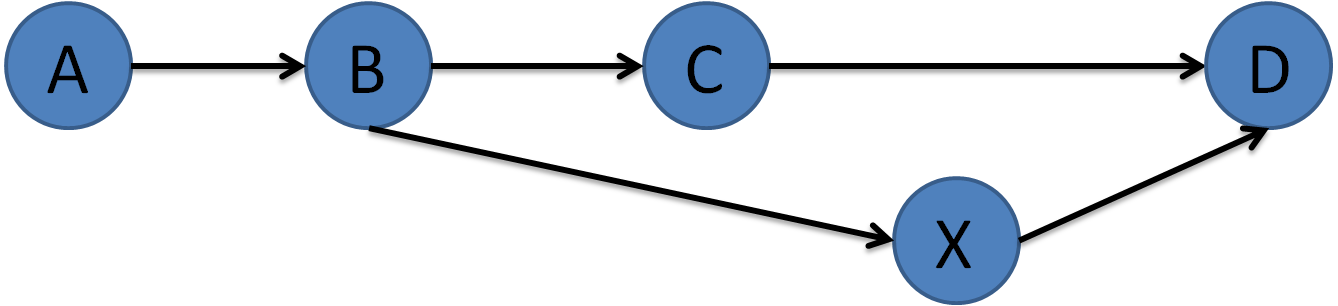
\includegraphics[width=3in]{Master.png}
\end{center}
\caption{The commit history graph when on the \texttt{master} branch}
\end{figure}

\noindent The following figure represents the commit history graph when on the \texttt{alt} branch:

\begin{figure}[h!]
\begin{center}

\includegraphics[width=3in]{Alt.png}
\end{center}
\caption{The commit history graph when on the \texttt{alt} branch}
\end{figure}

\newpage
%\vskip.25in
\noindent\textbf{Problem 2 (10 pts):}

\noindent Assume that you have created a new github repository at: 
\begin{center} 
\texttt{https://github.com/ssu7/PoemCollection.git}
\end{center} 
\newline The following GIT Bash commands will produce what the problem asks for:
\begin{lstlisting}
$ git config --global user.name "Steven" #Sets the user name
$ git config --global user.email "stevenemail@yahoo.com" #Sets the email of the user
$ mkdir hondacrv.git #Makes new git folder
$ cd hondacrv.git #Changes the directory to the git folder
$ git init #Initializes the git folder
$ git remote add Stanza1 git://github.com/nhlee/550400.stanza1.git #Creates alias for stanza 1
$ git remote add Stanza2 git://github.com/nhlee/550400.stanza2.git #Creates alias for stanza 2
$ git remote add Stanza3 git://github.com/nhlee/550400.stanza3.git #Creates alias for stanza 3
$ git pull Stanza1 master
$ vi main.txt #Add Title to Poem in VIM
$ git add .
$ git commit -m "Stanza1 Added"
$ git pull Stanza2 master
$ vi main.txt # Resolve Merge Conflict in VIM
$ git add .
$ git commit -m "Stanza2 Added"
$ git pull Stanza3 master
$ vi main.txt # Resolve Merge Conflict in VIM
$ git add .
$ git commit -m "Stanza3 Added"
$ git remote add origin https://github.com/ssu7/PoemCollection.git
$ git push origin master #Pushes main.txt to the previously setup github repository
\end{lstlisting}


%Assume that you are starting from ``scratch'' at the directory \verb+~/+.
%Provide a sequence of git/bash commands that yields a git folder and 
%\begin{itemize}
%\item configure your git with your name and your email address,
%\item set up an alias for each of the git remotes listed below:
%\begin{verbatim}
%git://github.com/nhlee/550400.stanza1.git 
%git://github.com/nhlee/550400.stanza2.git 
%git://github.com/nhlee/550400.stanza3.git 
%\end{verbatim}
%Assume that each remote contains exactly single commit with 
%a txt file for a single (different) stanza,
%\item pull to combine three stanzas of a poem,
%\item after the first pull, add the title of the poem,
%\item after the second and third pull, resolve the merge conflict,
%\item after resolving the third pull merge conflict, push the result
%  to your (newly created) remote repository. 
%\end{itemize}

\newpage
\noindent\textbf{Problem 3 (40 pts):}

\paragraph{} The issue of asynchronous collaboration on a class project is a common problem faced by many college students. git, a free and open source version control software, offers a possible solution to this issue. In the proposed situation, there are 4 students, A, B, C, and D, who will all be working on different portions of a LaTeX/Beamer presentation. The main problem to model in this situation is how to setup a GIT work flow process that minimizes the merge conflict resolutions. 

\paragraph{}We will assume that each student will only edit the section of the Beamer presenation in \texttt{main.txt} which they are responsible for. They will NOT edit any other sections. If their section requires additional LaTeX packages, each student will add the necessary packages to the preamble portion of \texttt{main.txt}. Under these assumptions, the preamble part of \texttt{main.txt} is the lone exogenous variable. The model does not attempt to study/explain this variable. The endogenous variables are how the different sections of the Beamer presentation (\emph{Introduction}, \emph{Problem Statement}, \emph{Timeline}, and \emph{Deliverables}) are edited and comitted using git. 

\paragraph{} One possible workflow process that could be employed in this situation uses a remote git repository with a \texttt{master} branch and 4 other branches, say \texttt{A}, \texttt{B}, \texttt{C}, and \texttt{D}, one for each student. In this workflow, each student will clone the remote git repository onto their computer and (i.e. create a local git repository). Each student will then edit/create their respective section of \texttt{main.txt} while commiting these changes to only their assigned branch in their local repository. After a student is satisfied with his/her section of \texttt{main.txt}, he/she can then merge his/her final local branch to his/her local \texttt{master} branch. After this the student will push both his/her local assigned branch to the corresponding remote assigned branch as well as push the local \texttt{master} branch to the remote \texttt{master} branch. After a student pushes his/her local \texttt{master} branch to the remote \texttt{master} branch, he/she will be responsible for merging their section into the existing file. Since each student only edits his/her respective section of \texttt{main.txt}, the merge process should be fairly straight-forward and easy. Each section of \texttt{main.txt} in the \texttt{master} branch of the remote repository should be empty up until the student who is responsible for that section pushes his/her version of the presentation to the \texttt{master} branch in the remote repository. A student will only need to check to see if his/her section has been added correctly, and that the other sections haven't been affected (which they shouldn't). The only portion of \texttt{main.txt} that this is not true of is the preamble portion in which case a merge conflict may arise. However merging this section should be easy as well; each student should keep what is in the preamble of the version in the remote repository and add in the changes they made. 

\paragraph{}Using this workflow, the \texttt{master} branch in the remote repository should be very clean: the only nodes that appear in the commit history should be when each student adds his/her finalized section of the presentation. This workflow also allows for edits and commits made by each student for their section of the presentation to be remembered through the commit history of the 4 student branches. This workflow also minimizes the number of merges that need to be made since only each student will only merge their contributions to the remote \texttt{master} branch only once.

\paragraph{} Another possible workflow process uses one remote group repository with a single \texttt{master} branch. Each student will again clone the remote repository onto their own computer and create a local repository. However in this workflow, each student will edit and commit changes directly to his/her local \texttt{master} branch and every so often push and merge these commits to the remote \texttt{master} branch. Students will continue doing this until they are all satisfied with their sections. 

\paragraph{} This workflow involves more pushes and merges to the remote \texttt{master} branch then necessary. Most of these merges should still be straight-forward since each student will only make changes to their own section of \texttt(main.txt} which does not overlap with any other section. However merges that involve the preamble portion will again require special attention since all 4 students can potentially change this portion of the LaTeX file. This workflow also mixes the commit histories of each section into the remote \texttt{master} branch's commit history which could potentially be very messy. This workflow also fails to utilize branching, which is a main feature of git.

\paragraph{} Because the first proposed workflow minimizes the number of times the students merge files, it is better than the second proposed workflow. Anytime a merge happens, there is a chance that a merge conflict will arise which then needs to be resolved. Therefore by mimimizing the total times the students merge files, the first proposed workflow in essence minimizes the potential number of merge conflicts that need to be resolved. Because the recommended workflow model minimizes merge conflicts, it, in theory, solves the previously formulated problem which was to develop a workflow strategy which minimizes merge conflict resolutions. 

\paragraph{} We can test the recommended workflow model to see if it is indeed better then the second workflow by  having 4 students working on a group presentation employ the recommended workflow scheme and having another group of 4 students use the second workflow scheme. Whichever group of students encounters less merge conflicts and has less trouble with merge conflict resolutions is the group that used the better workflow. If the group using the recommended workflow follows it precisely, then in a worst case scenario they will have 4 merge conflicts to resolve (once per student), where as the other group could potentially have far more merge conflicts. Therefore we can conclude that our recommended workflow does indeed minimize merge conflicts and is better than the other proposed workflow. 

%Consider a team of four students, say, $A$, $B$, $C$ and $D$, 
%who just started working 
%on writing a \texttt{latex/beamer} file, say \texttt{main.tex}, 
%for a class presentation of their work statement.  
%Assume that they do not wish to coordinate their schedules for a
%concurrent group meeting (both virtually and physically).  
%Assume that:
%\begin{itemize}
%\item $A$ is in charge of \emph{Introduction},
%\item $B$ is of \emph{Problem Statement}, 
%\item $C$ is of  \emph{Timeline},
%\item $D$ is of \emph{Deliverable} part of the presentation.  
%\end{itemize}
%In other words, their contributions to \texttt{main.tex} do not overlap.
%Then, 
%\begin{itemize}
%\item first, devise a work flow strategy for the team so that they can
%  collaborate asynchronously using \texttt{git},
%\item next, devise yet another \texttt{git} strategy different from your earlier
%  proposal.  
%\end{itemize}
%Finally,
%\begin{itemize}
%\item discuss the strength and weakness of each of your proposed strategies in terms of merge
%conflicts resolution,
%\item make the final recommendation.  
%\end{itemize}
%In order to answer this question, \emph{build}
%a mathematical model, \emph{following} the guideline from IMM. 
%Use Section 1.4 and Section 1.5 of IMM as \emph{role models}.    
%For example, you are to identify which variables  are exogenous 
%and which are endogenous.  More specifically, among other things, 
%in your model, is the preamble part of \texttt{main.tex} an endogenous 
%or exogenous variable?  
%Note also that in addition to this issue, there are other issues that
%you are to consider.  So, \emph{be sure to consult IMM}. 
\vskip0.25in
\noindent\textbf{Problem 4 (aka.\ Fair Play, 40 pts):}
Answer the following question:
\begin{verse}
Is the tennis game fair?
\end{verse}
Note that unlike Problem 3, this question is vaguely stated.
This is intensional, whence to begin, you will first need to clarify
what exactly your question is.
You may use the class discussion on this particular 
problem, but you \emph{may not} directly refer to our 
discussion.  Instead, formulate the model carefully but concisely in 
your own words.   

\vskip0.25in
\noindent\textbf{Final Remarks about Problem 3 \& Problem 4:} 
They are open-ended problems.  However, your scores will be determined
by how well do you follow the exposition style outlined by IMM and
WMA.  For both problems, your write-up should be 
\begin{itemize}
\item self-contained,
\item covering all four parts of Section 1.3 of IMM,
\item paying a particular attention to any causal relation that you
  might be investigating, following Chapter 3 of WMA,
\item answering questions that are explicitly asked in the problem statements.
\end{itemize}
For Problem 3, focus mostly on Step 2 and Step 3 of Section
1.3 of IMM.  For Problem 4, focus mostly on Step 1 and Step
2.  For each problem, minimum 1 pages and maximum 2 pages.
\end{document}
